\section{Introduction And Motivation}\label{sec:intro}
Modern industry is increasingly demanding function orientation, integration, and efficiency of novel materials and components. The material of choice for a growing number of applications is carbon fiber reinforced polymer (CFRP), which allows an integration of these continuously rising demands and increasingly replaces conventional materials such as aluminum or steel.
 CFRP materials have desirable characteristics such as high specific stiffness, high specific strength and high corrosion resistance. Moreover, CFRP materials show these characteristics at considerably lower weight. At the same time, highly complex and integrated components, which were previously impossible to manufacture may be produced from CFRPs. Primary structures and highly loaded components in aeronautics are one example. Typically, carbon fiber reinforced polymer components and more specifically CFRP laminates with endless carbon fibers as addressed in this work consist of two main components:
a matrix, which acts as a bonding component, and the reinforcements, which allow for achieving the desired characteristics. Various production processes are used to manufacture CFRP laminates. Most of these processes start with the reinforcement component, weaving individual carbon fiber bundles (yarn) into sheets of carbon fiber cloth in a predefined pattern. These sheets of woven carbon fiber cloth are also referred to as fabric and form the geometrical structure of the final CFRP materials. Depending on the requirements of the final component, fabrics may be stacked in multiple layers in similar or different orientation. Both the  alignment of fabrics and the weaving pattern of the individual carbon fiber bundles strongly influence the properties of the CFRP laminate. Resins are then integrated in the material system to fill the gaps in the fabric forming the matrix component. The main function of the matrix is to act as a bonding between the individual carbon fiber bundles. After curing, the production process of the CFRP laminate is finished.

The increasing share of CFRPs as well as the complexity of both material system and final component has generated a strong demand towards non-destructive testing (NDT) techniques for quality control~\cite{Red2012}. Ultrasonic testing (UT) is the most commonly used method for this purpose. While UT provides a quick and cost-efficient overview of the material, it also lacks resolution and may generate arbitrary results, e.g., due to the geometry of the component. Industrial 3D X-ray computed tomography (XCT, also referred to as 3DXCT or cone beam XCT) is increasingly applied for non-destructive testing of fiber reinforced polymers~\cite{Kastner2012}. In contrast to UT, XCT generates a highly detailed 3D volumetric representation of the scanned specimen. In cone beam XCT geometry the specimen is placed on a rotary table between X-ray source and detector. The X-rays passing through the specimen get attenuated by the materials present. By transferring the X-rays in a scintillator layer into visible light, the detector records the corresponding 2D attenuation image (penetration image). The specimen is rotated, recording at each angular step a 2D attenuation image to generate the full series of attenuation images of a $360^\circ$ rotation required for a complete reconstruction of the data volume ~\cite{heinzl-2008-thesis}. 
While cone beam XCT can reach voxel sizes below 500 $nm$ generating high resolution volume data for comprehensive and detailed analyses, unfortunately there is still a trade-off between viewport and image resolution. The magnification reached within an XCT scan is determined by the distances between source and specimen as well as source and detector. The magnification therefore directly influences both resolution and viewport: while higher resolutions decrease the viewport but show more details, lower resolutions allow for larger viewports and thus larger portions of the specimen.

In this work, we focus on datasets with larger viewports but
lower resolutions where the individual carbon fibers (filaments) are indiscernible or barely visible. Our domain experts are mainly interested in visualizing the geometric structures in the weaving pattern of fiber bundles in endless carbon fiber reinforced composites instead of high resolution studies of individual fibers.
%of short fiber reinforced composites as presented by Weissenbock2014 et al.~\cite{Weissenbock2014}.
Figure~\ref{fig:data-char} depicts our targeted dataset type. It shows the recurring fiber bundle pattern in the final CFRP laminate, the \textit{unit cell}.
Our work is motivated from the recent progress in two interrelated fields: Firstly, CFRP components have gained wide application in industry because of its superior material and physical properties in comparison to conventional materials~\cite{Karpat2012}. Secondly, recent developments of industrial 3D X-ray computed tomography (XCT) with regard to larger detectors, larger field of views, and better resolutions opened XCT for this new application area of non destructive testing for fiber reinforced components~\cite{Schilling2005}. 

While fiber bundles are now understood as highly important in determining component properties, the tools for visualizing the internal structure have not developed at the same pace.
To the best of our knowledge, there is no current work that can resolve simple queries such as:
\begin{itemize}[noitemsep]
	\item{ How to extract and visualize the geometric structure of a particular fiber bundle?}
	\item{ How to visualize the interaction between a particular pair of fiber bundles (weaving/braiding) or a unit cell?}
	\item{ Which fiber bundles show a particular orientation? }
	\item{ Which fiber bundles are of the same type of yarn? I.e. which bundles show similar sizes or diameters, which is the largest or smallest fiber bundle ?}
\end{itemize}

We demarcate the above queries into two parts: \textit{geometric structure} and \textit{spatial context}. Geometric structure refers to the shape, size, and orientation of a fiber bundle or a group of them. Spatial context refers to how two or more bundles interact with each other.It provides answers to questions such as: Are these bundles in contact at a particular position in the data? What are the relative orientations of the contacting bundles? 
Providing answers to the above queries from the volume renderings of XCT datasets or from visual inspection of particular 2D slices is non-trivial, even for experts. We present and evaluate a method which uses visualization techniques to gain insight into our data.
We interpret and advance techniques from diffusion tensor imaging to extract and visualize geometric structures from 3D X-ray computed tomography data of the woven carbon fiber reinforced composites. The main goal of this work is to expand the state of the art in non-destructive testing through visualization of composite structures in \textit{complete unit cells} of woven fabrics.
\begin{figure}[htb]
	\centering
	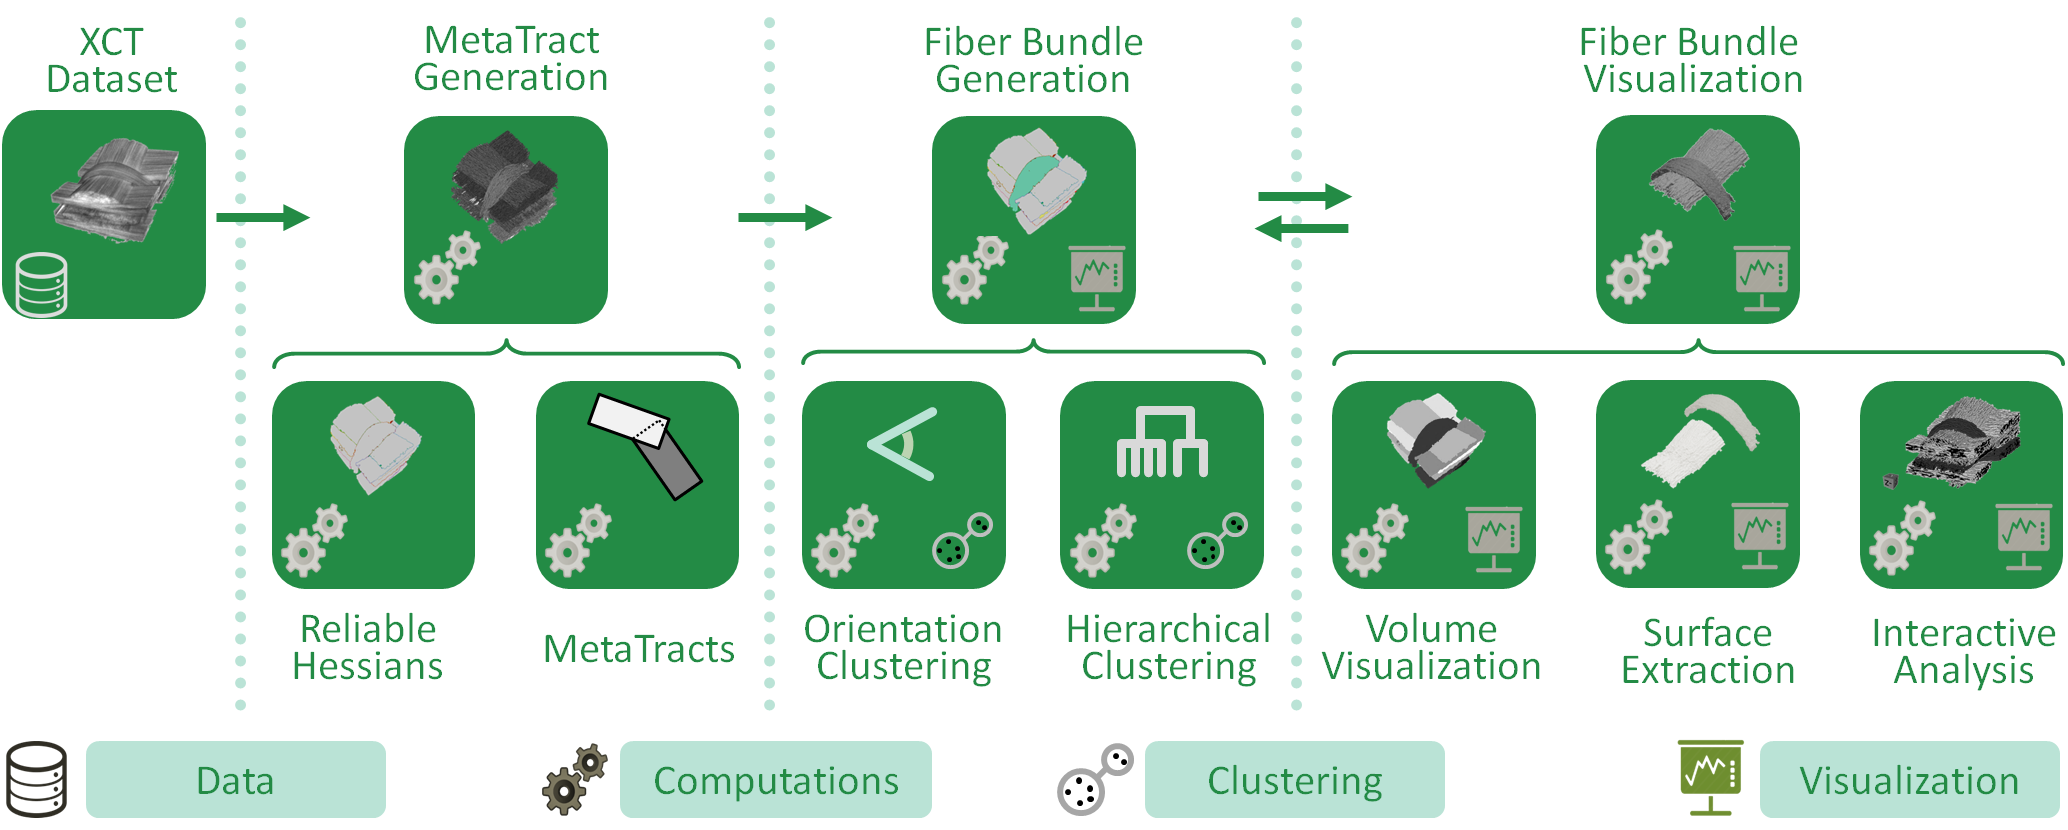
\includegraphics[width=\linewidth]{images/workflow_2.eps}
	\caption{Flow chart of the MetaTracts approach for fiber bundle extraction}
	\label{fig:flowchart}
\end{figure}
Figure~\ref{fig:flowchart} shows an over view of our approach.
Starting from XCT data, we first generate MetaTracts (see Sec.~\ref{sec:ext_mt}). Then we cluster the MetaTracts to generate and visualize fiber bundles (see Sec.~\ref{subsec:fiber-bundles}). We discuss the visualizations we created for our domain experts in Sec.~\ref{sec:vis}. Sec.~\ref{sec:results} describes our experimental results, Sec.~\ref{sec:param_choices} presents our parameter choices and  Sec.~\ref{sec:user_eval} summarizes the user evaluation of our method.
